\chapter{Introducción}

Los tumores cerebrales son una de las formas más letales de cáncer. Específicamente, los glioblastomas y sus variantes difusas son los más comunes y agresivos tipos de tumor del sistema nervioso central en adultos. Su alta heterogeneidad en apariencia, forma e histología los convierte en una de las patologías más difíciles de diagnosticar, de tratar y un reto para el campo de la imagen médica.

Desde el punto de vista de la ingeniería y la informática, vemos como sin duda la aplicación de técnicas de Visión por Computador es una de las máximas para la investigación en imagen médica en la actualidad. Sólo considerando su aplicación en el diagnóstico de enfermedades, desde 2008 el número de publicaciones promedio realizadas por año se ha incrementado notablemente tanto que actualmente es diez veces mayor que en sus inicios. 

Resultados notables como la inclusión de robots especializados para la cirugía \cite{cheng2022vinci} o buenos resultados en competiciones de ciencia de datos que replican la precisión médica en el diagnóstico mediante imagen \cite{bulten2022artificial} evidencian esta tendencia. El trabajo conjunto de personal médico e ingenieros promete seguir dando resultados que de forma separada eran inaccesibles.



\section{Objetivos}


Con este trabajo se persigue la creación de una arquitectura basada en aprendizaje profundo para equipar a un programa de uso médico, estudiarla y compararla junto a trabajos previos y estado del arte. Este programa tiene el objetivo de la ayuda en la evaluación del diagnóstico y pronóstico de un posible paciente de tumor cerebral y en caso afirmativo, la ayuda en la aplicación de la terapia por radiación. 

Se seguirá un planteamiento similar al seguido en la competición \textbf{BraTS: Brain Tumor Segmentation 2023} \cite{baid2021rsna} históricamente reconocida por ser un benchmark recurrente de las capacidades de las arquitecturas profundas en el campo de la imagen médica.

BraTS es una competición que se define como un conglomerado de diferentes tareas relevantes en el diagnóstico de los tumores cerebrales <<Cluster of Challenges>>. En 2023 dando especialmente importancia a la generalidad de un modelo que mantenga los resultados anteriores para pacientes más diversos (de diferente origen étnico y de diferentes edades) y con diferentes tipos de tumores. En concreto para 2023, se contemplaron las siguientes tareas por separado: segmentación de glioblastomas en adultos, segmentación de meningiomas en adultos, segmentación de tumores pediátricos, segmentación de tumores de pacientes de origen africano, generación de pruebas faltantes y generación de partes de la imagen.

De forma análoga a esta competición, se plantea conseguir dicho objetivo a partir de la resolución de las siguientes tareas.

\begin{enumerate}
	\item \textbf{Segmentación de los tumores.} 
	La segmentación de la lesión tumoral de los glioblastomas y los meningiomas.
	\item \textbf{Clasificación entre tipos de tumores.} Clasificación binaria entre glioblastomas y meningiomas. El programa indicará de qué tipo de tumor se trata.
	\item \textbf{Predicción de la evolución.} La segmentación a corto plazo de la más probable instancia futura a partir de la resonancia actual. Ya no solo se pretende dar una segmentación y clasificación que pudieran aportar valor en las decisiones médicas, sino predecir una nueva segmentación a partir de la resonancia apoyándose en casos similares y en la segmentación de la metástasis de la resonancia actual.
\end{enumerate}

A continuación, detallaremos de una forma más profunda la naturaleza de este planteamiento.

Sólo en los EEUU para 2024 se esperan 25400 nuevos casos de tumor cerebral. La supervivencia de estos a los cinco años es del $33.8 \%$ de los pacientes. \cite{cancerorg}

El cerebro no tiene terminaciones nerviosas. Los pacientes no sienten dolor a causa de un tumor cerebral por sí mismo, lo cual hace que no exista una alerta sobre el paciente que lo motive a buscar ayuda médica en las primeras fases de la patología. Generalmente, acaban buscando ayuda médica por la aparición de otros indicios relacionados difíciles de distinguir de otras patologías agudas y de menor transcendencia como visión borrosa, pérdida del control, etc. Además, los glioblastomas son tumores de muy rápido crecimiento pueden llegar a estar en una fase avanzada desde su inicio en tan solo 2-3 meses.

Por estos motivos, es común llegar tarde. Tomando mucha importancia el diagnóstico temprano para su superación. Con el objetivo de dar un diagnostico temprano se han introducido máquinas basadas en aprendizaje profundo. Así en este proyecto evaluaremos las capacidades del aprendizaje profundo para la segmentación de tumores. Prestando mayor interés a aquellos tumores que en sus inicios podrían pasar desapercibidos por el especialista humano, e incluso dar una segmentación de zonas potenciales que pueden aparecer nuevos tumores.

En general, los tumores cerebrales son difíciles de tratar y son resistentes a terapias convencionales usadas en otros tipos de cánceres como la quimioterapia debido a los desafíos que presenta el cerebro para tolerar ciertos químicos, transportar medicamentos dentro de él y la alta importancia que tiene en este órgano la optimización del uso de tratamientos que puedan ser invasivos. En otras palabras, el uso de tratamientos basados en la extirpación o en la medicación pueden ser arriesgados. Por tanto, el tratamiento más común de estos está basado en la radioterapia.

A la hora de aplicar un tratamiento de radioterapia siempre se tiene el objetivo de ser lo menos invasivo posible. Para ello, el médico debe ser lo más preciso posible en introducir la segmentación correcta en la que se aplicarán los rayos. 

Uno de los objetivos específicos para la ayuda en el tratamiento se basaría en el uso del modelo para automatizar esta tarea ya que podría suponer ahorrar costes en errores humanos y en tiempo a veces escaso para el personal médico cuya tarea se reduciría a corregir dicha segmentación. En nuestro caso, integrándolo en un programa de uso médico. 

Por otro lado, de forma general podemos interpretar este trabajo como un \textbf{sistema de apoyo a la decisión médica} ya que en ningún caso respecto el desarrollo actual de este problema se pretende sustituir la decisión final del personal médico. Aunque sí aprovechar las capacidades que puede ofrecer el aprendizaje profundo en un mejor diagnóstico a través de caracterizar mejor el tejido afectado: segmentándolo y clasificándolo.

Este sistema de apoyo a la decisión médica se plasmaría en una aplicación de escritorio que el personal médico pueda usar como paso intermedio entre la recogida de las imágenes del escáner y un posible tratamiento de radioterapia.


\section{Metodología}

\subsection{Conjunto de datos}

Una de las \textbf{limitaciones frecuentes en el campo de la imagen médica} es la poca disponibilidad de datos. En general y también para nuestro problema, las dificultades que se presentan a la hora de construir un conjunto de datos médico grande son:

\begin{enumerate}
	\item \textbf{Poca densidad de pruebas médicas.} A pesar de que la densidad de casos es alta, es frecuente que la cantidad de pruebas que se realizan sea mucho más baja. Especialmente, para datos médicos es frecuente encontrarse con pocos datos en magnitud con la necesidad de variabilidad en la muestra que tienen las técnicas típicas de optimización.
	
	\item \textbf{La desvinculación de los pacientes de sus datos}. El tratamiento de un dato médico siempre supone la eliminación de cualquier identificativo que ponga en riesgo la privacidad de este. Suponiendo un trabajo adicional para el personal médico que no siempre se puede asumir.
	
	\item \textbf{No existe una fuerte centralización de datos}. Al igual que los avances en imagen médica, el interés por la construcción de una base de datos única que recoja los máximo datos posibles es también reciente haciendo que en la actualidad la mayoría de los datos estén distribuidos en muchos centros médicos diferentes con formatos diferentes.
	
\end{enumerate}

Partimos del conjunto de datos \textbf{BraTS} y serán los que únicamente utilizaremos para todo el trabajo ya que son los únicos que se pueden encontrar en la red pidiendo un acceso a ellos de una forma simple e incluso podríamos decir legal.

Hasta nuestro conocimiento, \textbf{BraTS} es el mayor conglomerado de resonancias magnéticas en la actualidad para los desafíos que planteamos en este trabajo. Otros datasets usados por la comunidad para este problema como el incluido en \textbf{Medical Segmentation Decathlon} descubrimos que es un subconjunto de \textbf{BraTS}.


\textbf{BraTS} está patrocinado y organizado por la ASNR (American Society of Neurology), MICCAI (Medical Image Computing and Computer Assisted Intervention Society), National Cancer Institute, la Universidad de Pensilvania e Intel entre otros. 

\textbf{Los datos de BraTS son heterogéneos} ya no sólo externamente con diferentes tipos tumores (glioblastomas y meningiomas) y de pacientes de orígenes distintos y de diferentes edades sino también internamente con lesiones más y menos avanzadas en el tiempo (low- and high-grade) y con datos de multitud de centros que han sido escaneados con distintos escáneres.

Definiremos como nuestro conjunto de datos \textbf{$X$} a un conjunto de resonancias magnéticas cerebrales completas (resonancias con imágenes de todo el cerebro, no una parte). Este lo tenemos en formato \textbf{nii : Neuroimaging Informatics Technology Initiative (NIfTI)}. Con este formato podemos trabajar directamente con su versión comprimida en \textbf{gz: GNU ZIP}. Para ello, usaremos la librería \textbf{nibabel} que nos permite la lectura y conversión de cada resonancia a un array 3D de la librería NumPy de Python. Cada resonancia se despliega en un array 3D de dimensiones $240 \times 240 \times 155$. Siendo $155$ el número de imágenes del cerebro del paciente dividida en partes equidistantes. Cada imagen tiene una resolución $240 \times 240$.

Por otro lado, definimos el conjunto de etiquetas $Y$ como otro 3D-array de las mismas dimensiones que en el conjunto de datos $X$ donde se muestra la segmentación (Ground Truth) de los tumores.

En términos numéricos, contando solo los datos que tenemos sobre adultos tenemos $1251$ resonancias de glioblastomas de $1133$ pacientes diferentes y $1000$ resonancias de meningiomas de $944$ pacientes diferentes. Adicionalmente, tenemos resonancias de glioblastomas pediátricos y de adultos de origen africano que brindan de una distribución mucho más rica al dataset, aunque estos son una minoría siendo $99$ y $60$ respectivamente. 

\begin{figure}[!h]
	\centering
	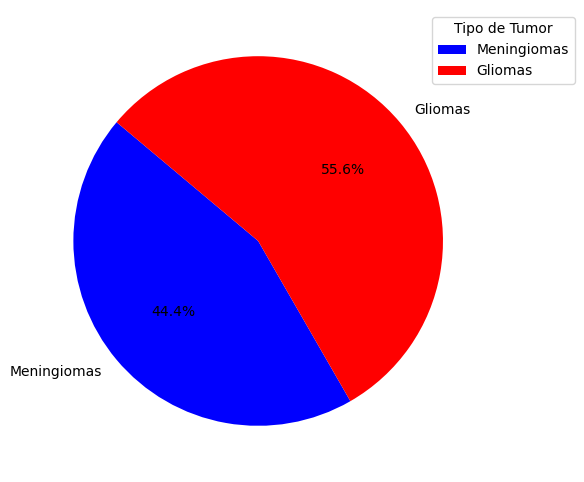
\includegraphics[width=0.8\linewidth]{imagenes/porcentajeGLIvsMEN.png}
	\caption{Porcentaje de Glioblastomas y Meningiomas en el conjunto de datos}
\end{figure}

Por otro lado, observamos los pacientes que tienen más de una resonancia versus los que tienen una única resonancia para caracterizar la cantidad de instancias temporales que tenemos en el dataset.
\\
\\
\\
\\
\\

\begin{figure}[!h]
	\centering
	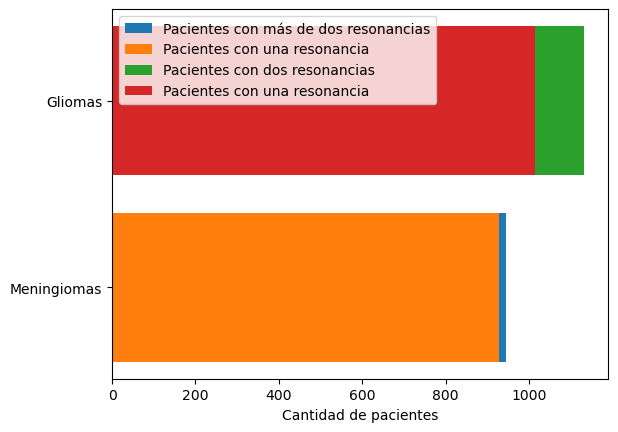
\includegraphics[width=0.8\linewidth]{imagenes/cantidadinstanciastemporales.png}
	\caption{Cantidad de instancias temporales en el conjunto de datos}
\end{figure}

En comparativa, observamos como la mayoría de pacientes no tienen más de una resonancia magnética, dejando sólo una cantidad de $118$ pacientes de glioblastoma y de $16$ pacientes de meningiomas con varias resonancias en el tiempo.

\subsubsection{Visualizado de datos}

A continuación, detallaremos más profundamente los datos haciendo algunas visualizaciones. 

Para todos los tumores $P$ del conjunto de datos tenemos distintos tipos de muestras según las características de la frecuencia empleada en la toma de la resonancia, \textbf{T1-weighted} o \textbf{T2-weighted}. \cite{labella2023asnrmiccai}

El tiempo de repetición (TR) es la cantidad de tiempo entre secuencias de pulsos sucesivas aplicadas al mismo segmento. El tiempo hasta el eco (TE) es el tiempo entre la llegada del pulso sobre el tejido y la recepción de la señal de eco.

Las imágenes ponderadas en T1 se producen utilizando tiempos TE y TR cortos. Por el contrario, las imágenes ponderadas en T2 se producen utilizando tiempos TE y TR más largos.

Las imágenes ponderadas en T1 muestran con más detalle la anatomía normal del tejido blando y la grasa. Las imágenes ponderadas en T2 muestran con más detalle el líquido y alteraciones (p. ej., tumores, inflamación, traumatismo). 

En resumen, tenemos cuatro 3D-arrays por resonancia magnética según frecuencia de señal y aplicando o no un agente de contraste:

\begin{enumerate}
	\item \textbf{T1N Pre-contrast T1-weighted} :  Resonancia en frecuencia T1 sin suministrarle ningún agente de contraste al paciente.
	\item \textbf{T1C Post-contrast T1-weighted} : Resonancia en frecuencia T1 suministrándole un agente de contraste al paciente.
	\item \textbf{T2W T2-weighted} : Resonancia en frecuencia T2 convencional.
	\item \textbf{T2F T2-weighted Fluid Attenuated Inversion Recovery} : Resonancia en frecuencia T2 en la que se anula la señal proveniente del líquido cefalorraquídeo.
\end{enumerate}

A continuación, observamos las imágenes producidas por una resonancia magnética en las diferentes pruebas para los dos tipos de tumores que tenemos.

\begin{figure}[!h]
	\centering
	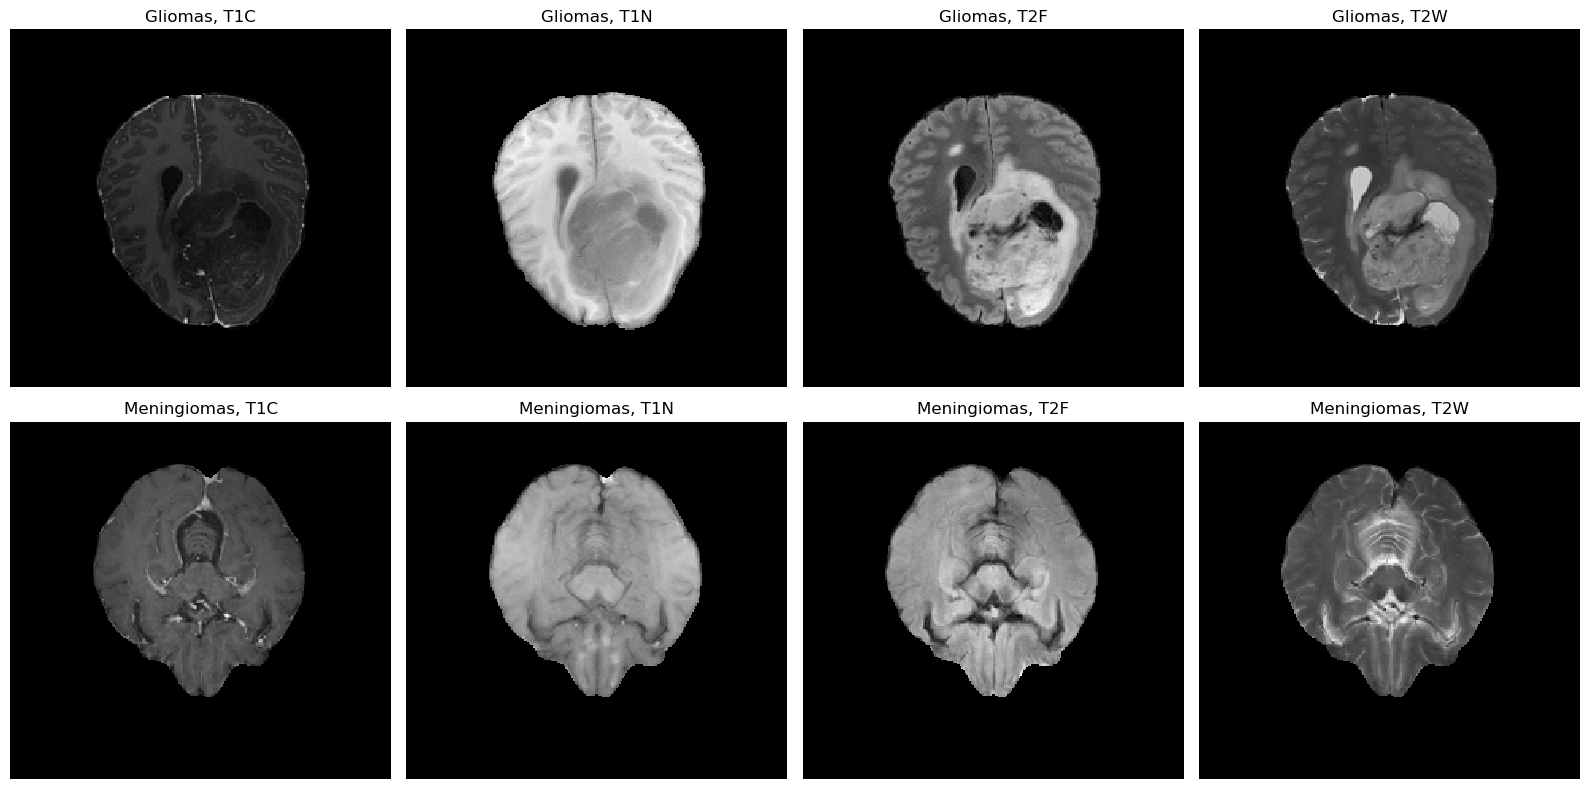
\includegraphics[width=1.0\linewidth]{imagenes/introduccion_imagenesMRI.png}
	\caption{Visualización de imágenes MRI de tumores en adultos de origen europeo y americano}
	\label{fig:visual0}
\end{figure}

Por otro lado, podemos observar algunas imágenes de las resonancias más específicas que tenemos, pediátrica y de adultos de origen africano.

\begin{figure}[!h]
	\centering
	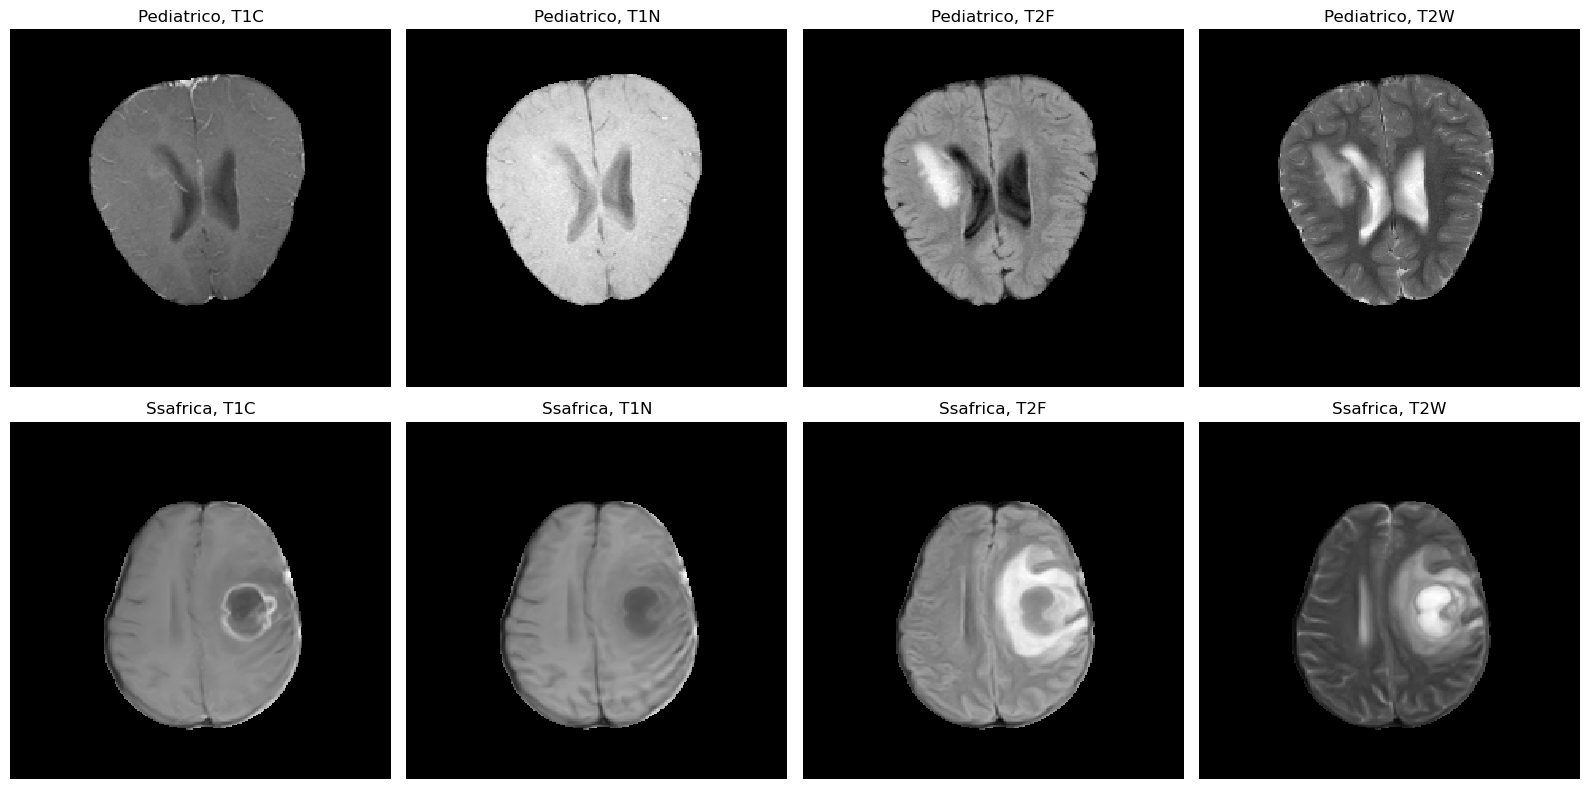
\includegraphics[width=1.0\linewidth]{imagenes/imgSSAPEDMRI.png}
	\caption{Visualización de imágenes MRI de glioblastomas en niños y adultos de origen africano}
	\label{fig:visual1}
\end{figure}

\newpage

A continuación, exploraremos el \textbf{etiquetado de las resonancias}, es decir, su segmentación realizada por el personal médico colaborador en \textbf{BraTS}.

La etiquetas de la segmentación pueden tomar cuatro valores, los del intervalo $[0, 3]$ que están relacionados con el tipo de tejido que segmentan. Tenemos tres tipos de tejidos que se relacionan con el valor de etiquetas en el array.

\begin{enumerate}
	\item \textbf{Etiqueta 0. Sano}: Tejido sano o la no existencia de tejido es etiquetado con $0$.
	\item \textbf{Etiqueta 1. NCR}: Tejido Necrótico. Núcleo del tumor tejido sin vida y usualmente reseco.
	\item \textbf{Etiqueta 2. ED}: Edema peritumoral. Tejido afectado por expansión del tumor generalmente acumulación de líquido y tejido sano desplazado. 
	\item \textbf{Etiqueta 3. ET}: Enhancing tumor. Tejido donde se encuentra la principal actividad de expansión del tumor. Área de actividad tumoral más agresiva o prolifera.
\end{enumerate}

Podemos ver la segmentación de las resonancias que se mostraron en \href{fig:visual0}{Figura 1.3} y \href{fig:visual1}{Figura 1.4}.
\begin{figure}[!h]
	\centering
	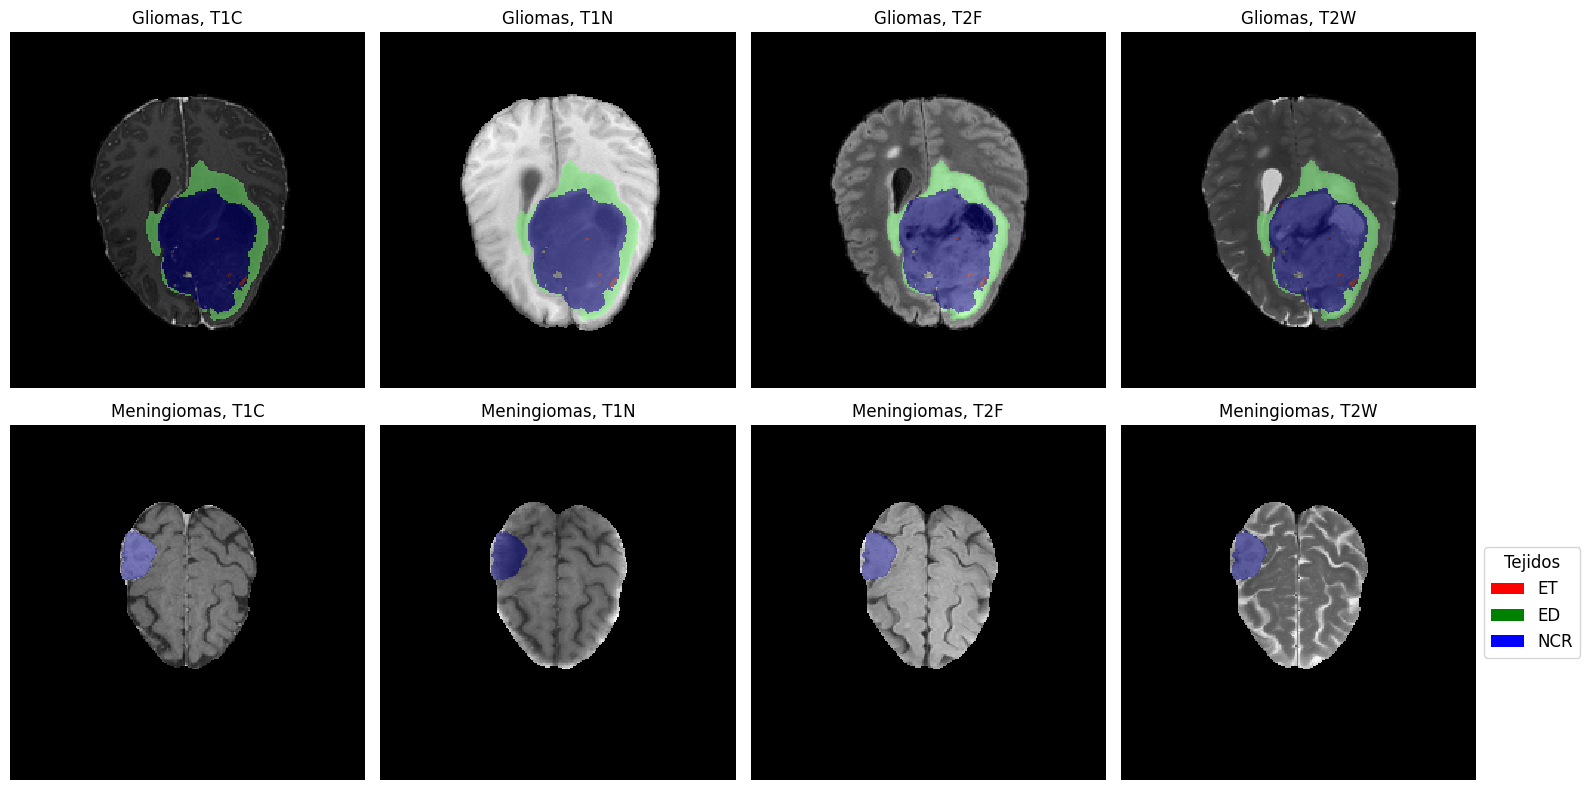
\includegraphics[width=1.0\linewidth]{imagenes/segimagenesMRI.png}
	\caption{Visualización de imágenes MRI de tumores en adultos de origen europeo y americano con su segmentación.}
\end{figure}

\begin{figure}[!h]
	\centering
	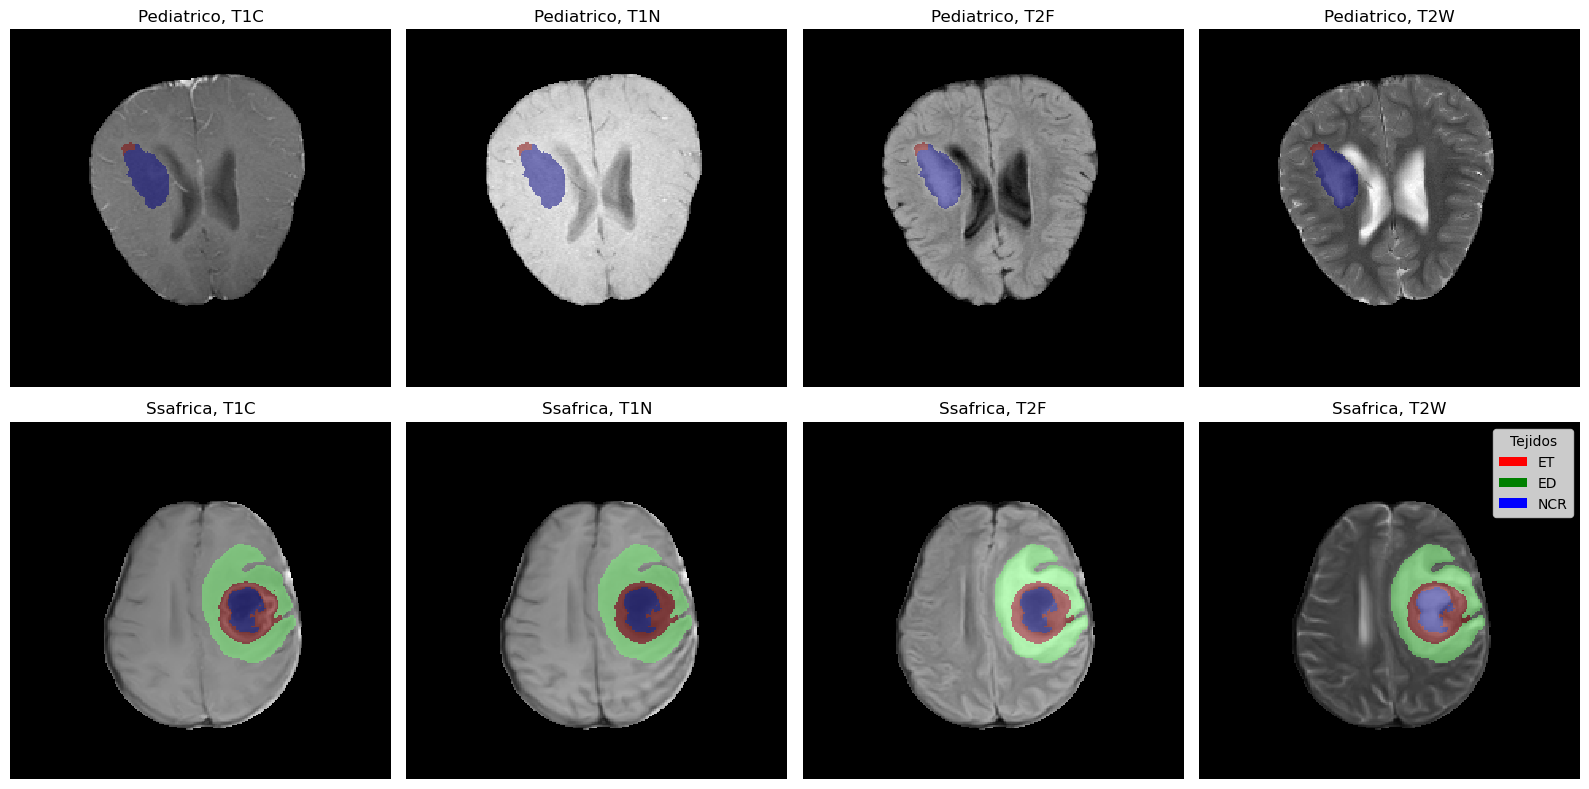
\includegraphics[width=1.0\linewidth]{imagenes/segimagenesSSAPEDMRI.png}
	\caption{Visualización de imágenes MRI de tumores en niños y adultos de origen africano con su segmentación.}
\end{figure}

\newpage
A continuación, exploraremos la \textbf{localización de los tumores} en todo el conjunto de datos. Buscando responder a la siguiente pregunta significativa para el trascurso del trabajo: ¿Existe alguna zona del cerebro especialmente afectada? Para responderlo podemos intentar visualizarlo. Crearemos un mapa de calor para los $150$ primeros slices marcando la presencia de la lesión, ponderaremos de forma lineal a los tejidos según su importancia.

\begin{figure}[!h]
	\centering
	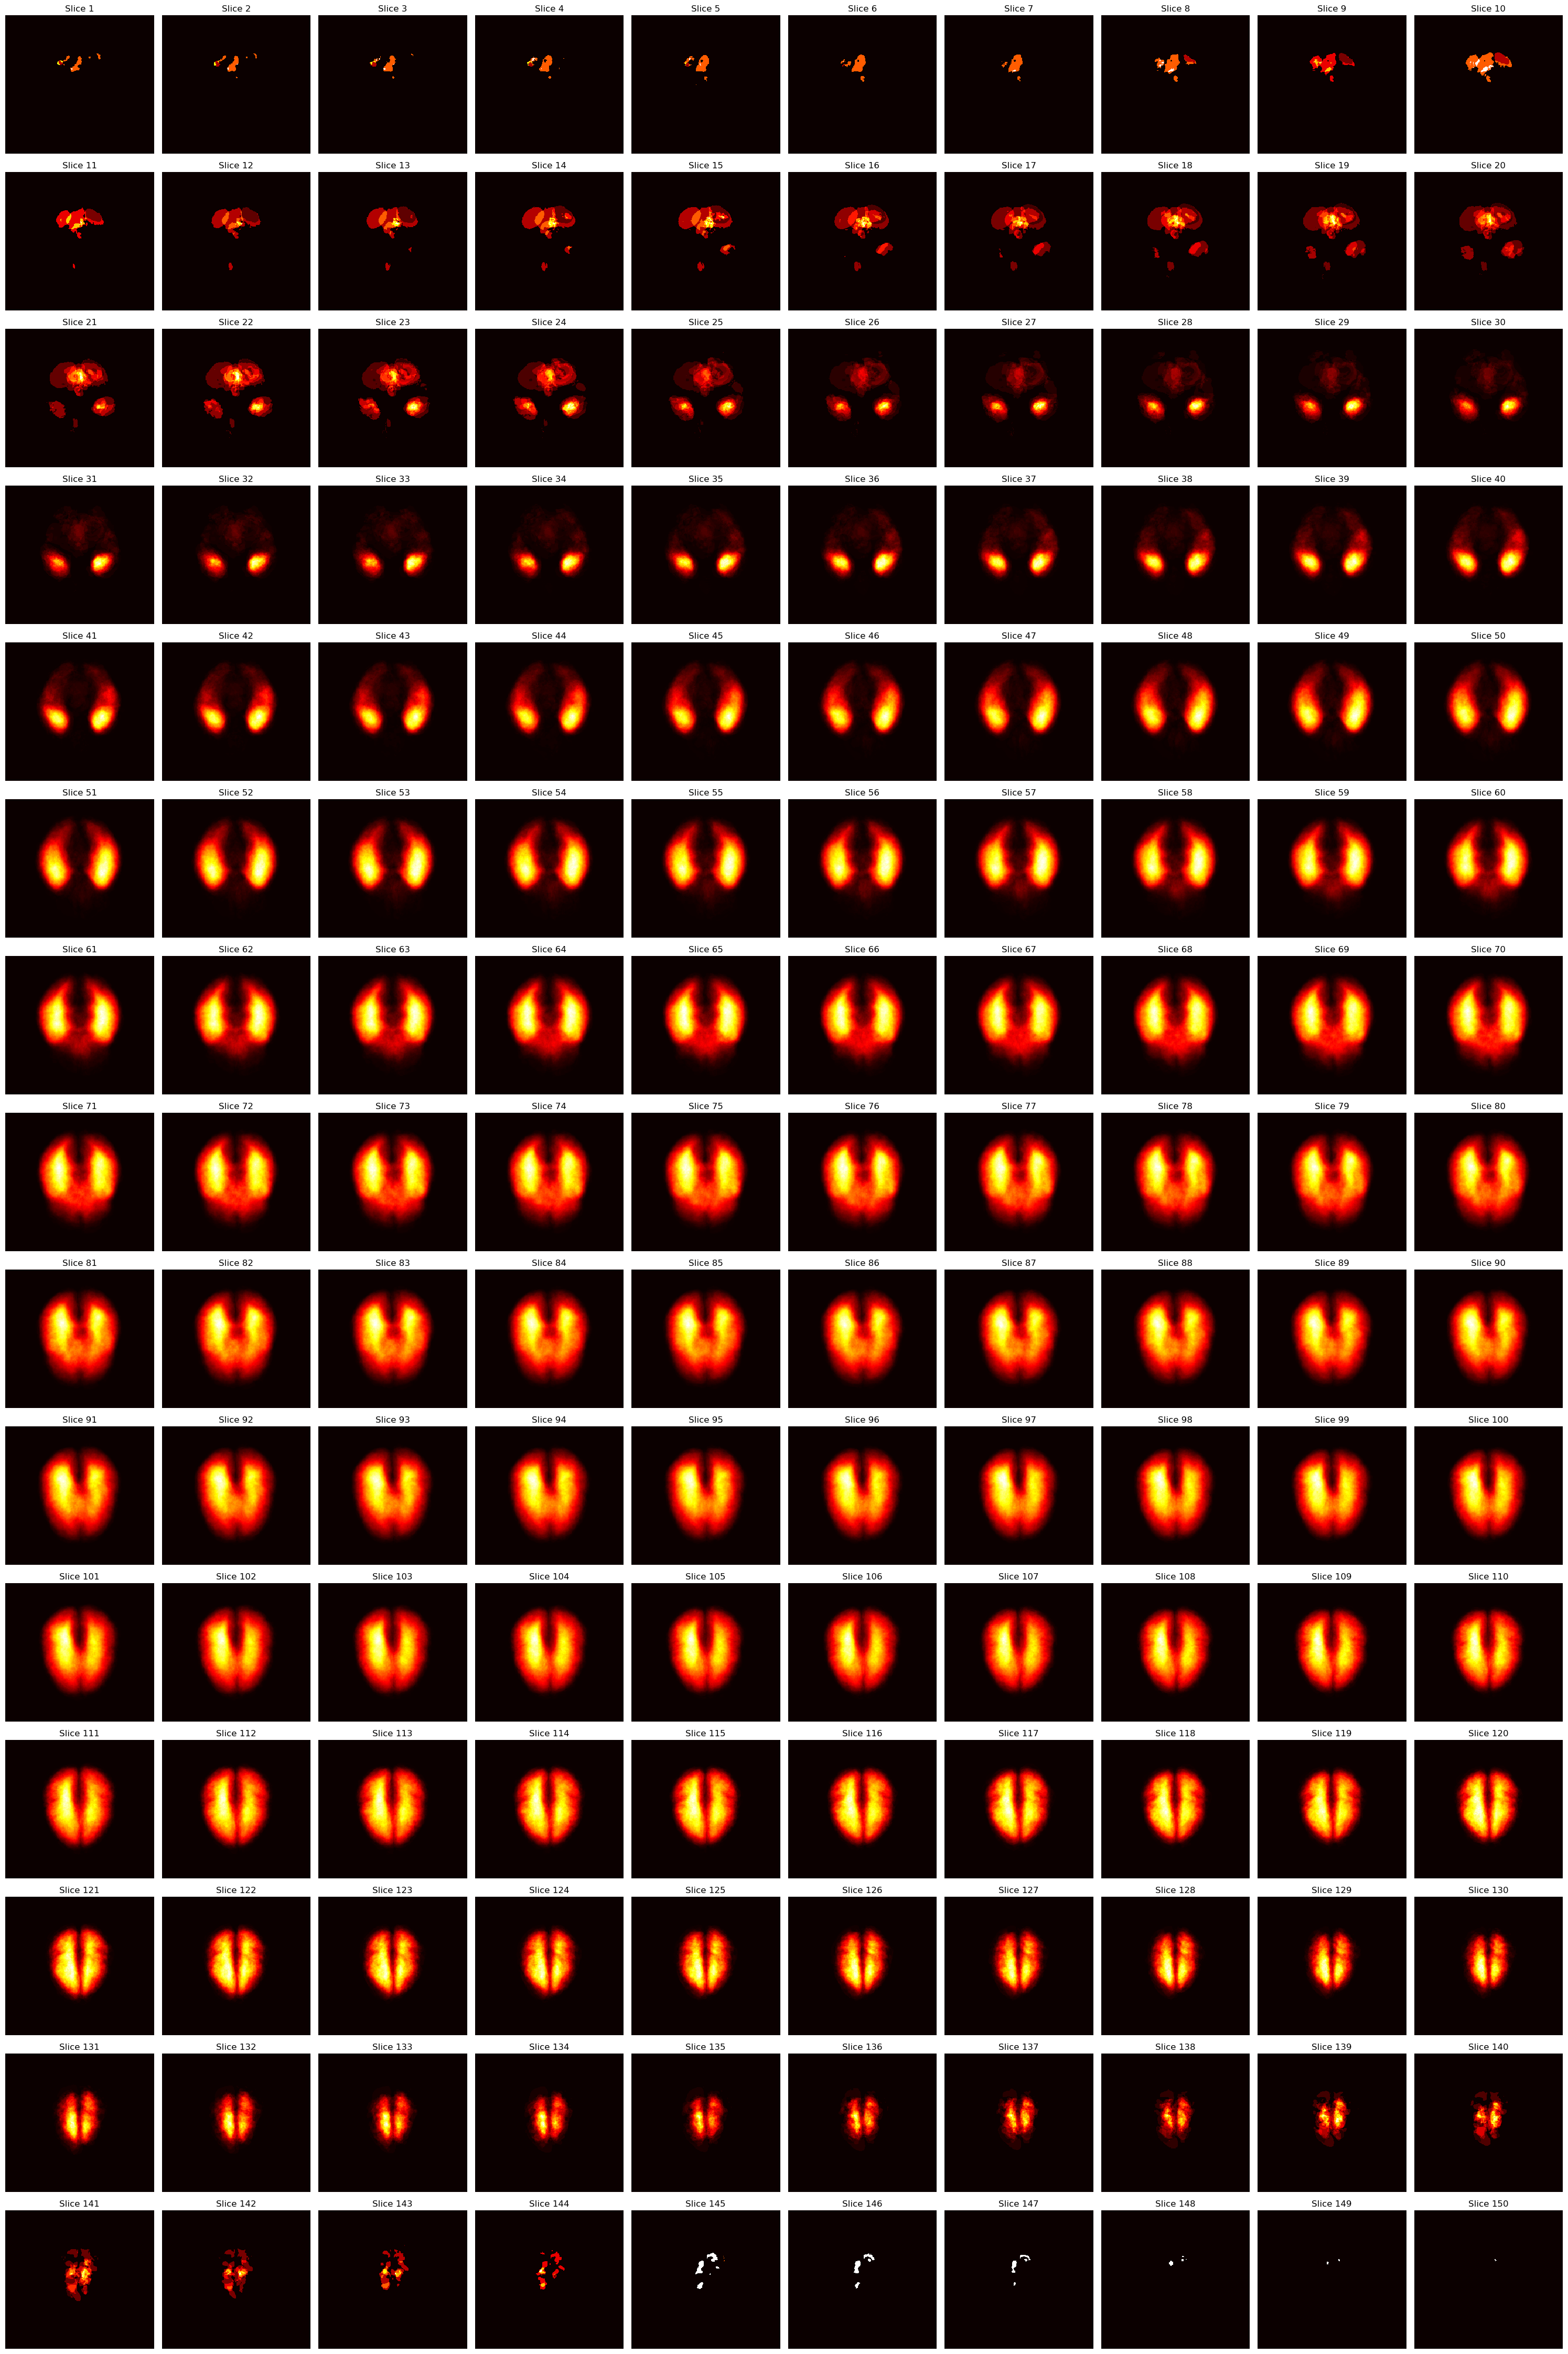
\includegraphics[width=1.0\linewidth]{imagenes/metodologia_heatmapsGLI.png}
	\caption{Distribución del tejido tumoral en Gliomas.}
\end{figure}

\begin{figure}[!h]
	\centering
	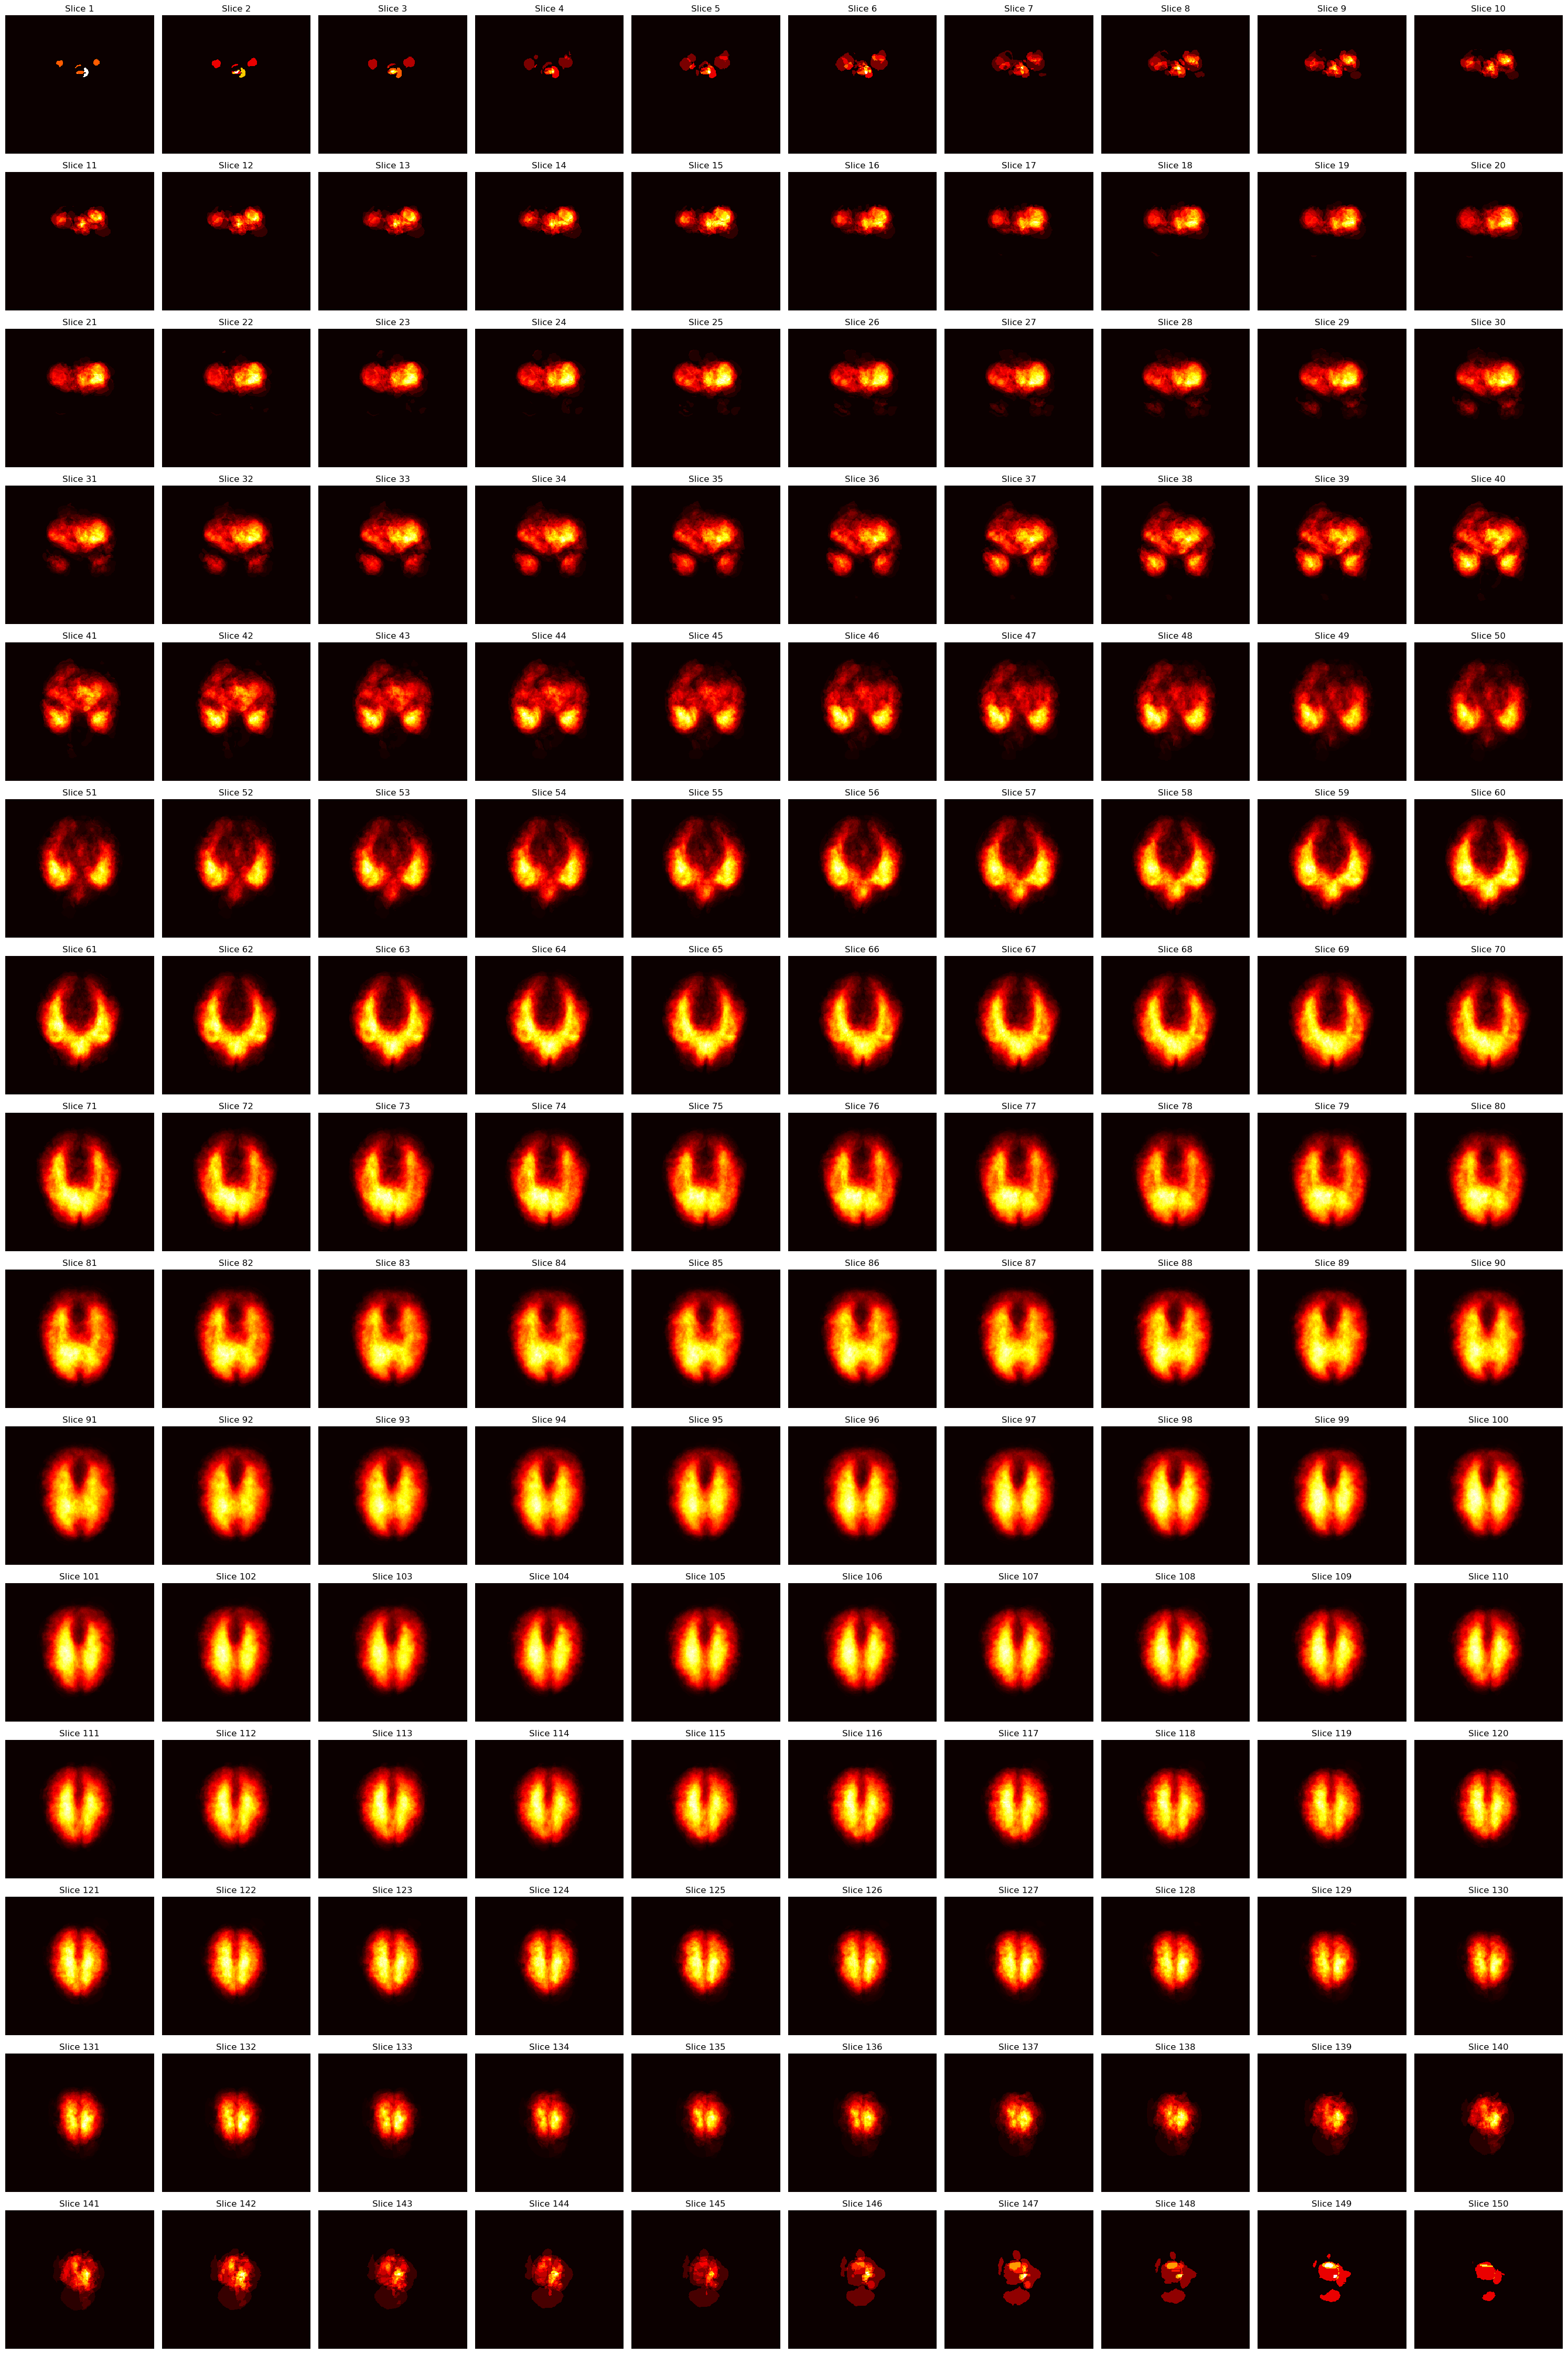
\includegraphics[width=1.0\linewidth]{imagenes/metodologia_heatmapsMEN.png}
	\caption{Distribución del tejido tumoral en Meningiomas.}
\end{figure}


Tras la visualización, no se observa una zona especialmente marcada ni en glioblastomas ni en meningiomas. Aunque sí ciertos detalles, como era de esperar en los primeros slices (que son de la base del cerebro) la zona de los meningiomas solo presenta tejido tumoral en la parte posterior esto es debido que a los meningiomas son tumores de desarrollo entre el cráneo y el cerebro, no habiendo ahí tejido posible de esta forma. Esto también puede explicar porque los gliomas tienen una distribución más centrada en los núcleos de los dos hemisferios del cerebro y los meningiomas más distribuido pero con una ligera tendencia en la parte frontal del cerebro donde más liquido cefalorraquídeo se concentra. A parte, de estos detalles íntegros a la naturaleza de estos tumores vemos como siguen una \textbf{localización independientemente distribuida}. 

\subsection{Línea de investigación}

 En este trabajo definiremos como línea base la construcción de un arquitectura encoder-decoder totalmente convolucional que se ajuste a los datos de entrenamiento. Para posteriormente utilizar el codificador y representación latente del autoencoder para todas las tareas. Conectándole:
 
 \begin{enumerate}
 	\item \textbf{Para clasificación} añadiendo una red densamente conectada. 
 	\item \textbf{Para segmentación}  un decodificador totalmente convolucional transformando la arquitectura en un autoencoder ResU-net (U-net con conexiones residuales).
 	\item \textbf{Para predicción} un decodificador basado en modelos sequence-to-sequence como los transformadores debido a la naturaleza secuencial que tienen diferentes resonancias de un mismo paciente en el tiempo.
 	
 \end{enumerate}
 
 La tarea de predicción sólo se planteará a nivel teórico por una baja existencia de datos con información temporal. 
 
\subsection{Planificación del trabajo}

A continuación, mostramos la planificación de llevar a cabo este trabajo en un entorno real a través de una tabla de Gram que recoja el presupuesto y tiempo dedicado a en cada fase del desarrollo de la investigación y de su software.

\begin{table}[H]
	\centering
	\begin{tabular}{|ccc|}
		\toprule
		\textbf{Tarea} & \textbf{Semanas} & \textbf{Presupuesto medio} \\
		\midrule
		Revisión del estado del arte & 1-2 & 300 \\
		Definición de línea de investigación & 1-2 & 300 \\
		Implementación de los experimentos & 1-2 & 300 \\
		Ejecución de los experimentos & 3-4 & 900 \\
		Validación de los experimentos & 1-2 & 310 \\
		Diseño de la interfaz & 1 & 200 \\
		Implementación de la interfaz & 1-2 & 300\\
		Documentación & 1 &  200 \\
		\hline
		\textbf{Total} & 10-16 &  2810 \\
		\bottomrule
	\end{tabular}
	\caption{Planificación del trabajo con tiempos y presupuesto.}
	\label{tabla:planificacion}
\end{table}

El presupuesto medio necesario ha sido calculado lo que costaría pagar a un becario durante ese tiempo  para esa tarea asumiendo que el becario cobra \textbf{800} euros al mes más el coste del uso del hardware empleado en los experimentos. 

Para el calculo del hardware no asumimos que usamos las gráficas gratuitas de Kaggle sino que la alquilamos en Lambda Cloud con un precio de uso de $\approx 5$ euros por hora.


\subsection{Metodología de desarrollo}

En este trabajo nos intentaremos ajustar lo máximo posible a una metodología de desarrollo ágil, \textbf{SCRUM}. Contemplando las siguientes características a cumplir.

\begin{enumerate}
	\item \textbf{Enfoque en roles y procesos}: SCRUM define roles. En nuestro caso, la tutora líder del proyecto (tomando las decisiones estructurales) y el alumno implementador y solucionador (llevándolo a la práctica y tomando el resto de decisiones). También define procesos estructurados como las reuniones de planificación de sprint, la revisión de sprint y la retrospectiva. Que se traducen en las tutorías y comunicación proporcionado durante el desarrollo del proyecto.
	
	\item \textbf{Iterativo e incremental}: SCRUM se basa en iteraciones cortas (sprints) para desarrollar de manera incremental. En nuestro comenzando por clasificación y posteriormente por segmentación. Así como seguir la planificación de trabajo dispuesta anteriormente, informando de ello.
	
	\item \textbf{Flexibilidad en las prácticas técnicas}: SCRUM permite adaptarse. Esta característica es muy importante en este proyecto ante pruebas sin éxito o cambios de enfoque que sean necesarios.
\end{enumerate}